% Hahn decomposition of the signed density f(x)=x on [-1,1].
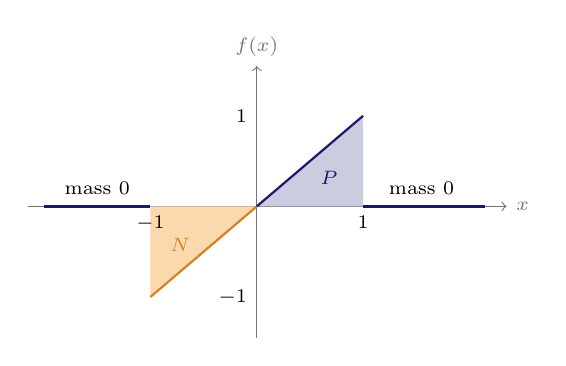
\begin{tikzpicture}[x=1.35cm,y=1.15cm]
  \draw[black!55,->] (-2.15,0) -- (2.35,0) node[right,font=\scriptsize] {$x$};
  \draw[black!55,->] (0,-1.45) -- (0,1.55) node[above,font=\scriptsize] {$f(x)$};
  \fill[BurntOrange!28] (-1,0) -- (-1,-1) -- (0,0) -- cycle;
  \fill[MidnightBlue!22] (0,0) -- (1,1) -- (1,0) -- cycle;
  \draw[BurntOrange!85!black,thick] (-1,-1) -- (0,0);
  \draw[MidnightBlue,thick] (0,0) -- (1,1);
  \draw[MidnightBlue,thick] (-2,0) -- (-1,0);
  \draw[MidnightBlue,thick] (1,0) -- (2.15,0);
  \node[font=\scriptsize,BurntOrange!85!black] at (-0.72,-0.42) {$N$};
  \node[font=\scriptsize,MidnightBlue] at (0.68,0.32) {$P$};
  \node[font=\scriptsize,below] at (-1,0) {$-1$};
  \node[font=\scriptsize,below] at (1,0) {$1$};
  \node[font=\scriptsize,left] at (0,-1) {$-1$};
  \node[font=\scriptsize,left] at (0,1) {$1$};
  \node[font=\scriptsize,above] at (-1.5,0.02) {mass $0$};
  \node[font=\scriptsize,above] at (1.55,0.02) {mass $0$};
\end{tikzpicture}
